\documentclass[
]{jss}

%% recommended packages
\usepackage{orcidlink,thumbpdf,lmodern}

\usepackage[utf8]{inputenc}

\author{
Søren B. Vilsen\\Department of Mathematical Sciences, Aalborg University
}
\title{Random weight neural networks in \proglang{R}: The \pkg{RWNN}
package}

\Plainauthor{Søren B. Vilsen}
\Plaintitle{Random weight neural networks in R: The RWNN package}
\Shorttitle{\pkg{RWNN}: Random Weight Neural Networks}


\Abstract{
This paper serves as an introduction to the \pkg{RWNN} package. The
\pkg{RWNN} package implements random weight neural networks. The methods
are implemented using a combination of \proglang{R} and \proglang{C++}
offsetting the heavier computation and estimation to \proglang{C++}
through the \pkg{Rcpp} and \pkg{RcppArmadillo} packages. While
implementations of random weight neural networks exist other
\proglang{R} packages, these focus on the simplest possible variant of
the random weight neural network and cover only very specialised use
cases of these networks. Besides a general purpose implementation of
random weight neural networks, the \pkg{RWNN} package also includes
common variants such as deep RWNN and sparse RWNN, as well as ensemble
methods using random weight neural networks as the base learner.
Furhtermore, the \pkg{RWNN} packages also includes more sophisticated
methods for initialising the random weights, as well as methods for
pruning both the number of weights and the number of neurons in the
network.
}

\Keywords{random weight neural networks, regularisation, ensemble
learning, Bayesian
computation, \proglang{R}, \pkg{Rcpp}, \pkg{RcppArmadillo}}
\Plainkeywords{random weight neural networks, regularisation, ensemble
learning, Bayesian computation, R, Rcpp, RcppArmadillo}

%% publication information
%% \Volume{50}
%% \Issue{9}
%% \Month{June}
%% \Year{2012}
%% \Submitdate{}
%% \Acceptdate{2012-06-04}

\Address{
    Søren B. Vilsen\\
    Department of Mathematical Sciences, Aalborg University\\
    Skjernvej 4A,\\
9220 Aalborg East\\
  E-mail: \email{svilsen@math.aau.dk}\\
  URL: people.math.aau.dk/\textasciitilde svilsen\\~\\
  }


% tightlist command for lists without linebreak
\providecommand{\tightlist}{%
  \setlength{\itemsep}{0pt}\setlength{\parskip}{0pt}}



%% preamble

\usepackage[utf8]{inputenc}
\usepackage[british]{babel}

\usepackage{amsmath, amssymb, bm, booktabs}





\begin{document}



\hypertarget{introduction}{%
\section{Introduction}\label{introduction}}

Neural networks, and variants thereof, have seen a massive increase in
popularity in recent years. This has largely been due to the flexibility
of the neural network architecture, and their accuracy when applied to
highly non-linear problems. However, due to the highly non-linear nature
of the neural network architecture, estimating the weights of these
networks using gradient based optimisation (i.e.~back-propagation), can
be slow and does not guarantee a globally optimal solution. In order to
combat these problems, various simplifications of the feed forward
neural network (FFNN) architecture have been proposed, including random
weight neural networks (RWNNs). They were first introduced in the early
1990's under the name random vector functional links (RVFL)
\citep[\citet{Pao1994}]{Schmidt1992}, and a simplified version was
re-discovered under the name extreme learning machines (ELM)
\citep{Huang2006} in the mid 2000's. The general idea of RWNNs is to
keep the randomly assigned weights of the network between the
input-layer and the last hidden-layer fixed, and focus on estimating the
weights between the last hidden-layer and the output-layer. In the case
of regression, this simplification makes estimating the output weights
of a RWNN equivalent to estimating the weights of a (regularised) linear
model. Theoretically RWNNs show similar universal approximation
properties as their FFNN counterparts, i.e.~as the number of neurons
tends towards infinity the RWNN should be able to approximate any
function arbitrarily well (placing only loose assumptions on the
activation function). However, practically the number of neurons needed
for this approximation to be acceptable may not be feasible for a
particular application. Therefore, extensions of RWNNs have been
proposed limiting the number of neurons in favour of deeper
architecture, as seen in deep RWNN \citep{Henriquez2018} and ensemble
deep RWNN \citep{Shi2021}, or in favour of sparse unsupervised
pre-training of the weights, like sparse RWNN \citep{Zhang2019}.

Implementations of RWNNs already exist in \proglang{R} through the
packages \pkg{nnfor} \citep{nnfor} and \pkg{elmNNRcpp}
\citep{elmNNRcpp}, both focusing on the simpler ELM architecture. Both
implementations allow for a varying number of neurons in the
hidden-layer, as well as the specification of the activation function,
but are limited to a single hidden-layer with no functional link between
the input- and output-layers. The \pkg{nnfor} package was designed for
using ELMs to handle time-series data and allows for forecasting at
different temporal frequencies using the \pkg{thief} package.
Furthermore, it allows for estimation of the output-weights using
Moore-Penrose inversion, \(\ell_1\)-regularisation, and
\(\ell_2\)-regularisation. The \pkg{elmNNRcpp} package is the successor
to \pkg{elmNN} package \citep{elmNN} re-implemented in \proglang{C++}
through \pkg{Rcpp} and \pkg{RcppArmadillo} \citep[\citet{RcppA}]{Rcpp}.
The package is a standard implementation of the ELM architecture for
both regression and classification. The package allows the user to
specify the leakage of the implemented relu activation function, as well
as the tolerance of the Moore-Penrose inversion used to estimate the
output-weights.

\pkg{RWNN} is a general purpose implementation of RWNNs in \proglang{R}
\citep{R} focusing on both regression and classification problems. The
\pkg{RWNN} package allows the user to create an RWNN of any depth, set
the number of neurons and activation functions in each layer, choose the
sampling distribution of the randomly assigned weights, and choose
whether the output weights should be estimated by either Moore-Penrose
inversion, \(\ell_1\)-regularisation, or \(\ell_2\)-regularisation. RWNN
is implemented in C++ through \pkg{Rcpp} and \pkg{RcppArmadillo}; along
with the standard RWNN implementation the following variants have also
been included:

\begin{itemize}
\tightlist
\item
  \textbf{ELM} (extreme learning machine) \citep{Huang2006}: A
  simplified version of an RWNN without a link between the input and
  output layer (this is also the default behaviour of the RWNN
  implementation).
\item
  \textbf{deep RWNN} \citep{Henriquez2018}, \citep{Shi2021}: An RWNN
  with multiple hidden layers, where the output of each hidden-layer is
  included as features in the model.
\item
  \textbf{sparse RWNN} \citep{Zhang2019}: Applies sparse auto-encoder
  (\(\ell_1\) regularised) pre-training to reduce the number non-zero
  weights between the input and the hidden layer (the implementation
  generalises this concept to allow for both \(\ell_1\) and \(\ell_2\)
  regularisation).
\item
  \textbf{ensemble deep RWNN} \citep{Shi2021}: An ensemble extension of
  deep RWNNs using the output of each hidden layer to create an ensemble
  of RWNNs, each hidden-layer being used to create a seperate prediction
  of the target.
\end{itemize}

Furthermore, the \pkg{RWNN} package also includes general
implementations of the following ensemble methods (using RWNNs as base
learners):

\begin{itemize}
\tightlist
\item
  \textbf{Stacking} \citep{Wolpert1992}, \citep{Breiman1996a}: Stack
  multiple randomly generated RWNN's, deep RWNN's, or sparse RWNN's and
  estimate their contribution to a weighted ensemble using \(k\)-fold
  cross-validation.
\item
  \textbf{Bagging} \citep{Breiman1996b}, \citep{Breiman2001},
  \citep{Xin2021}: Bootstrap aggregation of RWNN's, deep RWNN's, or
  sparse RWNN's creates a number of bootstrap samples, sampled with
  replacement from the training-set. Furthermore, as in random forest,
  instead of using all features when training each RWNN, a subset of the
  features are chosen at random.
\item
  \textbf{Boosting} \citep{Friedman2001}: The boosting implementation is
  based on residual boosting using RWNN's, deep RWNN's, or sparse RWNN's
  as the base learner.
\end{itemize}

As RWNN's will inevitably include a lot of randomly generated features,
to improve their computational and memory efficiency, the \pkg{RWNN}
package also includes methods for pruning the number of weights and
neurons using magnitude, mutual information, and Fisher information.

Lastly, the \pkg{RWNN} package also includes a simple method for grid
based hyperparameter optimisation, where \(k\)-fold cross-validation is
applied to the training-set to find the hyperparameters yielding the
smallest cross-validation error on a user defined grid (similar to the
\pkg{tune} function found in the package \pkg{e1071} \citep{e1071}).

The remainder of the paper is structured as follows: Section \ref{RWNN}
introduces the general idea of RWNNs, this is followed by the method of
estimating the output weights, and an outline of each of the implemented
RWNN variants. The utility of the \pkg{RWNN} package is shown in Section
\ref{EX} applying different RWNN variants to a series of examples.
Lastly, a conclusion is found in Section \ref{CON}.

\hypertarget{RWNN}{%
\section{Random Weight Neural Networks}\label{RWNN}}

RWNN's are simplifications of FFNN's, where the weights between the
input-layer and the hidden-layers are kept fixed after being randomly
initialised, i.e.~only the weights between the last hidden-layer and the
output-layer are estimated during the training process. Furthermore, a
direct link (also called a functional link) between the features and the
output may be included; when the link is active, the RWNN can be seen as
a concatenation of the original features, and a random non-linear
transformation of these features. Using this simplification, assuming
the loss is the squared loss, and that the activation function is linear
(i.e.~the identity function), then estimation of the output-weights
simplifies greatly, as it becomes equivalent to estimating the weights
in (regularised) multiple linear regression. The general structure of
RWNN's with a single hidden-layer can be seen in Figure \ref{fig:rwnn},
where the dashed red lines indicate the functional link.

\begin{CodeChunk}
\begin{figure}[ht!]

{\centering 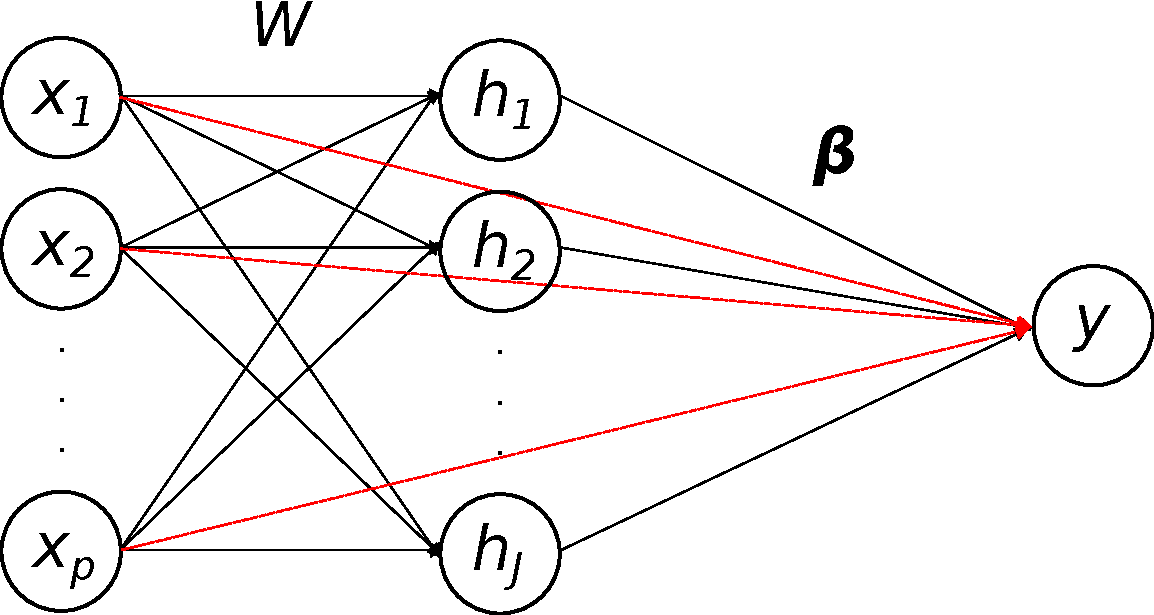
\includegraphics[width=0.6\linewidth]{./Figures/RWNN} 

}

\caption[Graph representation of a random weight neural network (RWNN) with funcitonal link between the input and the output layer]{Graph representation of a random weight neural network (RWNN) with funcitonal link between the input and the output layer.}\label{fig:rwnn}
\end{figure}
\end{CodeChunk}

\hypertarget{rwnn}{%
\subsection{RWNN}\label{rwnn}}

Given a sample of \(N\) observations,
\(\mathcal D = \{(\boldsymbol x_n, y_n)\}_{n = 1}^N\), where
\(\boldsymbol x_n\) is \(p\) dimensional vector of features and \(y_n\)
is the target, of observation \(n\), the output of the \(j\)'th neuron
in the hidden layer is: \begin{equation}
    h_{nj} = f\left(\sum_{i = 1}^p w_{ij} x_{ni} + w_{0}\right), \label{eq:hidden}
\end{equation} where \(f\) is the activation function, \(w_0\) is the
bias, and \(w_{ij}\) is the weight between the \(i\)'th feature and the
\(j\)'th neuron. If the hidden-layer contains \(J\) neurons, then the
vector of features transformed by the hidden layer, denoted
\(\boldsymbol h_{n}\), can be simplified to: \begin{equation} 
    \boldsymbol h_n = \boldsymbol f\left(W \boldsymbol{x}_n + w_0 \boldsymbol{1}_{J}\right), 
\end{equation} where \(\boldsymbol{1}_{J}\) is a vector of one's of
dimension \(J\).

Assuming the activation in the output-layer is linear, then the expected
response of the \(n\)'th observation is: \begin{equation}
    \hat{y}_n = \boldsymbol d^T_n \boldsymbol \beta,
\end{equation} where \(\boldsymbol d_n\) is either the output of the
hidden-layer (i.e.~\(\boldsymbol d_n = \boldsymbol h_n\)), or the
concatenation of input-layer and the output of the hidden-layer
(i.e.~\(\boldsymbol d_n = [\boldsymbol h_n^T \; \boldsymbol x_n^T]^T\)),
dependent on whether the functional link is inactive or active,
respectively. Furthermore, in the following, references to the the
functional link will be avoided when possible, and the dimension of the
features \(\boldsymbol d_n\) will simply be denoted \(l\).

The \pkg{RWNN} package allows the user to specify the number of neurons
in the hidden-layer, and the activation function among those listed in
Table \ref{tab:activation}.

\begin{table}[ht!]
\caption{\label{tab:activation}The name, specification, function, and range for each of the activation functions implemented in the \pkg{RWNN} package.}
\centering
\begin{tabular}{lllc}
\toprule
\textbf{Name} & \textbf{Specification} & \textbf{Function} & \textbf{Range} \\ 
\midrule
Identity & \texttt{identity} & $f(x) = x$ & $(-\infty, \infty)$ \\[5pt]
Bent identity & \texttt{bentidentity} & $f(x) = \dfrac{\sqrt{x^2 + 1} - 1}{2} + x$ & $(-\infty, \infty)$ \\[10pt]
Gaussian & \texttt{gaussian} & $f(x) = \exp(-x^2)$ & $(0, 1]$ \\[7pt]
Hyperbolic tangent & \texttt{tanh} & $\text{tanh}(x) = \dfrac{\exp(x) - \exp(-x)}{\exp(x) + \exp(-x)}$ & $(-1, 1)$ \\[10pt]
Rectified linear unit & \texttt{relu} & $f(x) = \max\{0, x\}$ & $[0, \infty)$ \\[5pt]
Sigmoid & \texttt{sigmoid} & $f(x) = \dfrac{1}{1 + \exp(-x)}$ & $(0, 1)$ \\[10pt]
Sigmoid linear unit & \texttt{silu} & $f(x) = \dfrac{x}{1 + \exp(-x)}$ & $[-0.278..., \infty)$ \\[10pt]
Softsign & \texttt{softsign} & $f(x) = \dfrac{x}{1 + |x|}$ & $(-1, 1)$ \\[10pt]
Softplus & \texttt{softplus} & $f(x) = \ln(1 + x)$ & $(0, \infty)$ \\[5pt] 
SQNL & \texttt{sqnl} & $f(x) = \left\{\begin{array}{ll} -1, & \text{if } x < -2 \\[3pt] x + \frac{x^2}{4}, & \text{if } -2 \leq x < 0 \\[3pt] x - \frac{x^2}{4}, & \text{if } 0 \leq x < 2 \\[3pt] 1, & \text{if } 2 \leq x \end{array} \right.$ & $[-1, 1]$ \\[15pt] 
Squared RBF & \texttt{sqrbf} & $f(x) = \left\{\begin{array}{ll} 1 - \frac{x^2}{2}, & \text{if } |x| \leq 1 \\[3pt] \frac{(2 - |x|)^2}{2}, & \text{if } 1 < |x| < 2 \\[3pt] 0, & \text{if } |x| \geq 2 \end{array} \right.$ & $[0, 1]$ \\[5pt]
\bottomrule
\end{tabular}
\end{table}

Thus, if the weights of the hidden-layer can be assumed to be known,
then the expected response of an RWNN is identical to that of a linear
model. However, before estimating the weights, it it is necessary to
determine the weights of the hidden-layer.

\hypertarget{HST}{%
\subsubsection{Sampling hidden-weights}\label{HST}}

In RWNN's, the standard approach to determining the weights between in
input- and hidden-layer(s), is to sample the weights randomly from a
uniform distribution limited to an appropriate interval for the
activation function used in the hidden-layer. However, as shown by
\citep{Wang2017}, using complete random initialisation might not be the
best approach when generating these weights, as it tends to require a
large number of neurons in the hidden-layer for the RWNN to have
generalisability. Therefore, they introduced two alternatives to the
random initialisation: quasi-random numbers, and random orthogonal
projections. The three methods have all been implemented in the
\pkg{RWNN} package, and are outlined below:

\begin{itemize}
\tightlist
\item
  \textbf{Random initialisation}: The weights between the input- and
  hidden-layer, \(w_{ij}\), are sampled independently from the same
  distribution, \(\mathcal D(\theta)\). The \pkg{RWNN} package is set-up
  to facilitate the use of any (including user defined) distribution to
  sample these weights. However, if nothing is specified, it defaults to
  a uniform distribution on the interval \([-1;1]\),
  i.e.~\(w_{ij}\sim\mathcal U([-1;1])\) for all \(i\) and \(j\).
\item
  \textbf{Quasi-random initialisation}: Quasi-random numbers have the
  distinct advantage, when compared to \emph{true} random numbers, that
  they will cover the domain of interest faster and more evenly. Thus,
  when using quasi-random numbers, the space can be more effectively
  explored, leading to a higher performance using less neurons in the
  hidden-layer. The \pkg{RWNN} package allows for the use of Halton and
  Sobol' sequences to generate quasi-random numbers by using the
  \proglang{R} package: \pkg{randtoolbox} \citep{randtoolbox}. If
  nothing is specified, it defaults to creating quasi-random numbers on
  the cube \([-1;1] \times [-1;1]\).
\item
  \textbf{Random orthogonal initialisation} (default): The idea is
  similar to that of random initialisation, but instead of using the
  randomly initialized weights directly, it uses an orthonormal basis of
  the sampled weights. The method used in the \pkg{RWNN} package
  corresponds to Algorithm 1 of \citep{Wang2017}.
\end{itemize}

\hypertarget{EST}{%
\subsubsection{Estimating output-weights}\label{EST}}

Given a matrix of features, \(D\), (i.e.~a matrix where the \(n\)'th row
contains \(\boldsymbol d_n^T\)) and a vector containing the targets,
\(\boldsymbol y\), the output-weights \(\boldsymbol \beta\) can be found
by minimising sum-of-squared errors (SSE): \begin{equation}
    \hat{\boldsymbol{\beta}} = \underset{\boldsymbol{\beta}}{\text{argmin}} \Big\{ || \boldsymbol{y} - D\boldsymbol{\beta}||_2^2\Big\}. \label{eq:ssq}
\end{equation}

In cases where \(N > l\), the solution to this system of equations can
be found by the normal equation, as: \begin{equation}
    \hat{\boldsymbol{\beta}}^{(ols)} = (D^T D)^{-1}D^T\boldsymbol{y}. \label{eq:ols}
\end{equation}

However, when the number of columns of \(D\) is bigger than the number
of observations (i.e.~\(l >> N\)), this optimisation problem becomes
ill-posed. In such cases, the two most common approaches, to estimating
the output-weights, are Moore-Penrose pseudoinverse and regularisation.

Using Moore-Penrose pseudoinverse
\citep[\citet{PenroseInv}]{BjerhammarInv}, \(D^+\), the solution to the
optimisation problem is given by: \begin{equation}
    \hat{\boldsymbol \beta}^{(pseudo)} = D^+ \boldsymbol y.
\end{equation}

Regularisation of the SSE, seen in Eq. \eqref{eq:ssq}, is achieved by
penalising the size of the output-weights. This penalisation is usually
performed using either the \(\ell_1\) or \(\ell_2\)-norm, creating the
following optimisation problem: \begin{equation}
    \hat{\boldsymbol{\beta}}^{(reg)} = \underset{\boldsymbol{\beta}}{\text{argmin}} \Big\{ || \boldsymbol{y} - D\boldsymbol{\beta}||_2^2  + \lambda||\boldsymbol{\beta}||_q^q \Big\}, \label{eq:rsse}
\end{equation} where \(q \in \{1, 2\}\), and \(\lambda\) is a
penalisation constant. The penalisation constant should be chosen such
that it minimises the out-of-sample error (using e.g.~\(k\)-fold
cross-validation during the training process).

Estimating of the weights differs slightly dependent on the choice of
\(q\):

\begin{itemize}
\item
  \underline{$\boldsymbol{q = 1}$}:\newline  The optimisation problem in
  Eq. \eqref{eq:rsse} is equivalent to performing lasso-regression
  \citep{SanLasso}, \citep{TibLasso}. Unlike ridge-regression
  (\(q = 2\)) it is not possible to find a closed form solution to the
  optimisation problem and, thereby, the lasso estimated output-weights,
  \(\hat{\boldsymbol{\beta}}^{(lasso)}\). However, it has been shown by
  \citep{CoordLasso}, that \(\hat{\boldsymbol{\beta}}^{(lasso)}\) can be
  found using coordinate descent.
\item
  \underline{$\boldsymbol{q = 2}$}:\newline  The optimisation problem in
  Eq. \eqref{eq:rsse} is equivalent to performing ridge-regression on
  the concatenated features, instead of the input features, and the
  solution can be found as \citep{ridgeReg}: \begin{equation}
  \hat{\boldsymbol \beta}^{(ridge)} = \left(D^TD + \lambda I_{l}\right)^{-1}D^T\boldsymbol y,
  \end{equation} where \(I_{l}\) is the identity matrix of size \(l\).
\end{itemize}

\hypertarget{deepRWNN}{%
\subsection{Deep RWNN}\label{deepRWNN}}

Extending FFNN's from a single hidden-layer to \(K\) hidden-layers will
barely change the governing equation of each neuron; assuming
\(h_{ni}^{(0)}\) is the \(i\)'th feature \(x_{ni}\) and that the number
of neurons in the \(k\)'th layer is \(J^{(k)}\), then the output of the
\(j\)'th neuron in the \(k\)'th layer for the \(n\)'th observation, is
given by: \begin{equation}
    h_{nj}^{(k)} = f^{(k)}\left(\sum_{i = 1}^{J^{(k - 1)}} w^{(k)}_{ij} h_{ni}^{(k - 1)} + w^{(k)}_{0}\right), \label{eq:hidden2} 
\end{equation} where \(f^{(k)}\) is the activation function,
\(w^{(k)}_0\) is the bias, and \(w^{(k)}_{ij}\) is the weight between
the \(i\)'th neuron and the \(j\)'th neuron in the \(k\)'th layer for
\(k = 1, ..., K\). Using vector notation this is simplified to:
\begin{equation}
    \boldsymbol h_n^{(k)} = \boldsymbol f^{(k)}\left(W^{(k)} \boldsymbol{h}^{(k)} + w^{(k)}_0 \boldsymbol{1}_{k}\right),
\end{equation} where \(\boldsymbol{1}_k\) is a vector of one's of
dimension \(J^{k}\).

Using deep FFNN's as starting point, when creating deep RWNN's two
approaches can be taken to predicting the target: (1) use the output of
just the last hidden-layer, or (2) concatenate the outputs of all \(K\)
hidden-layers. The graphical interpretation of the difference between
the two approaches can be seen on the left and right-hand sides of
Figure \ref{fig:deeprwnn}, respectively.

\begin{CodeChunk}
\begin{figure}[ht!]

{\centering 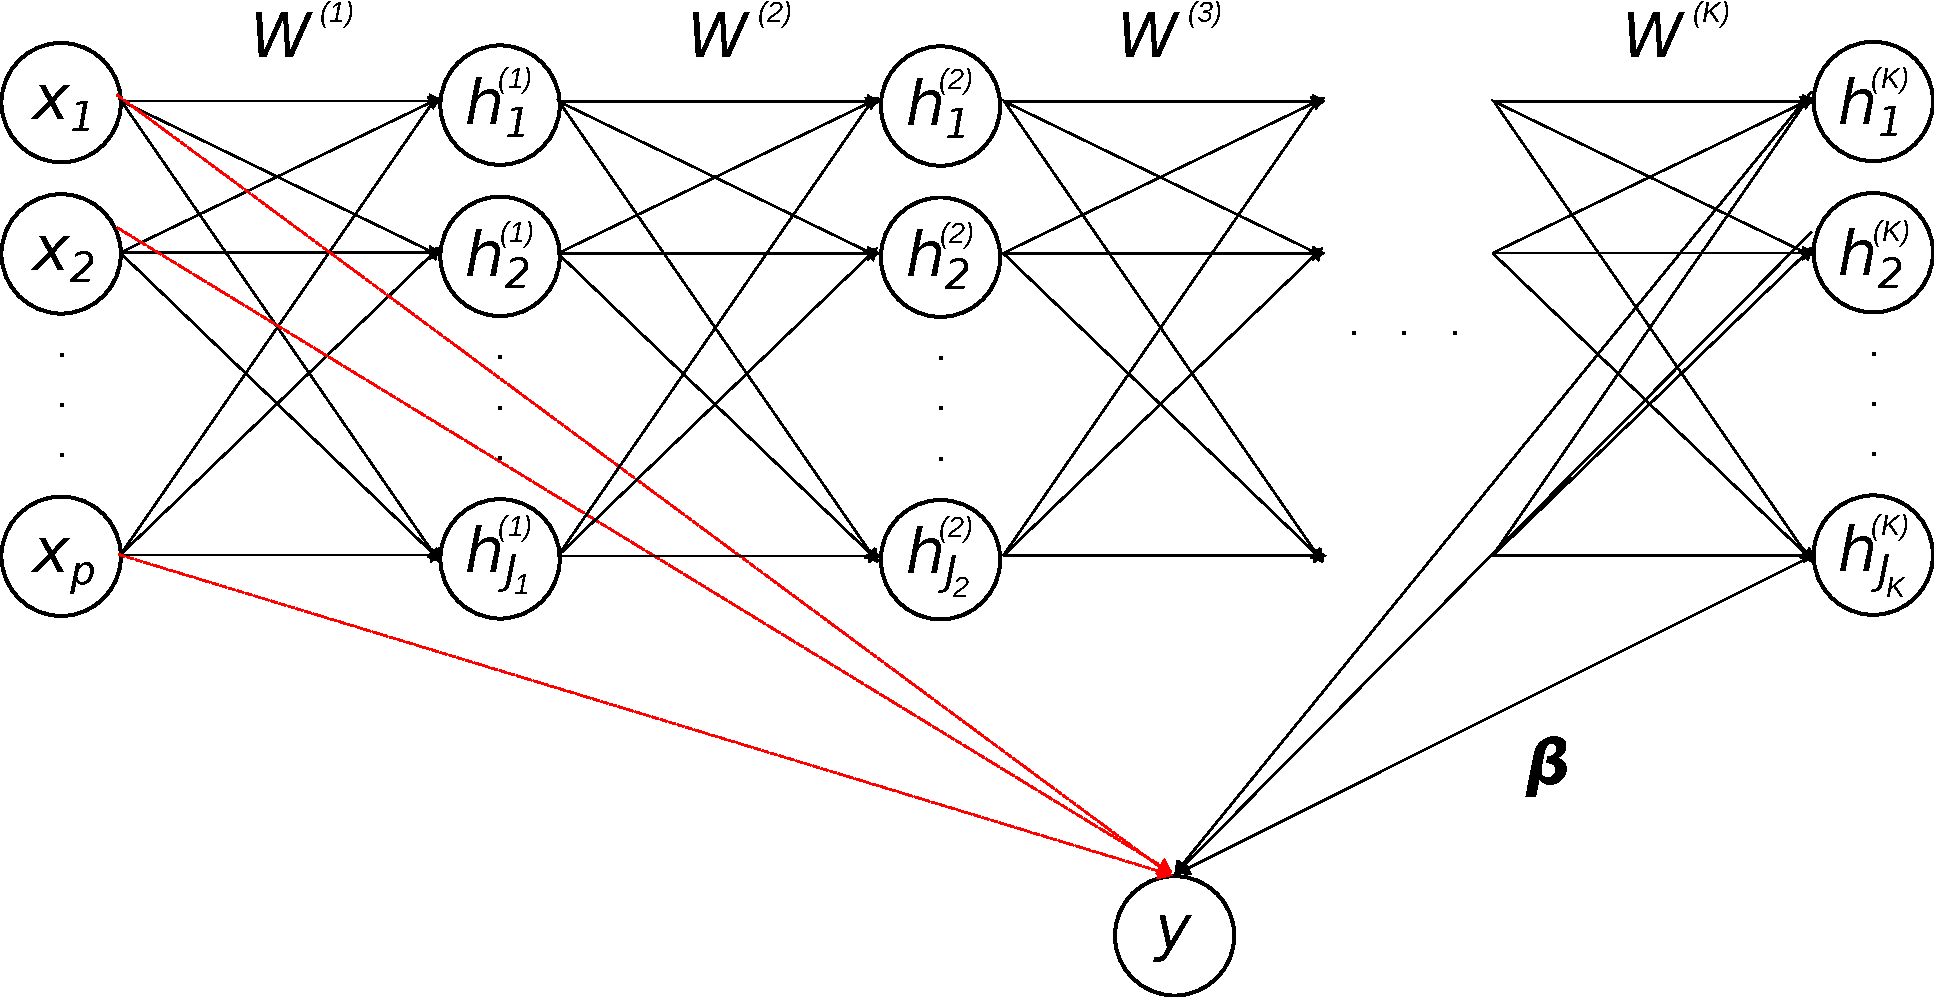
\includegraphics[width=0.45\linewidth]{./Figures/deepRWNN} 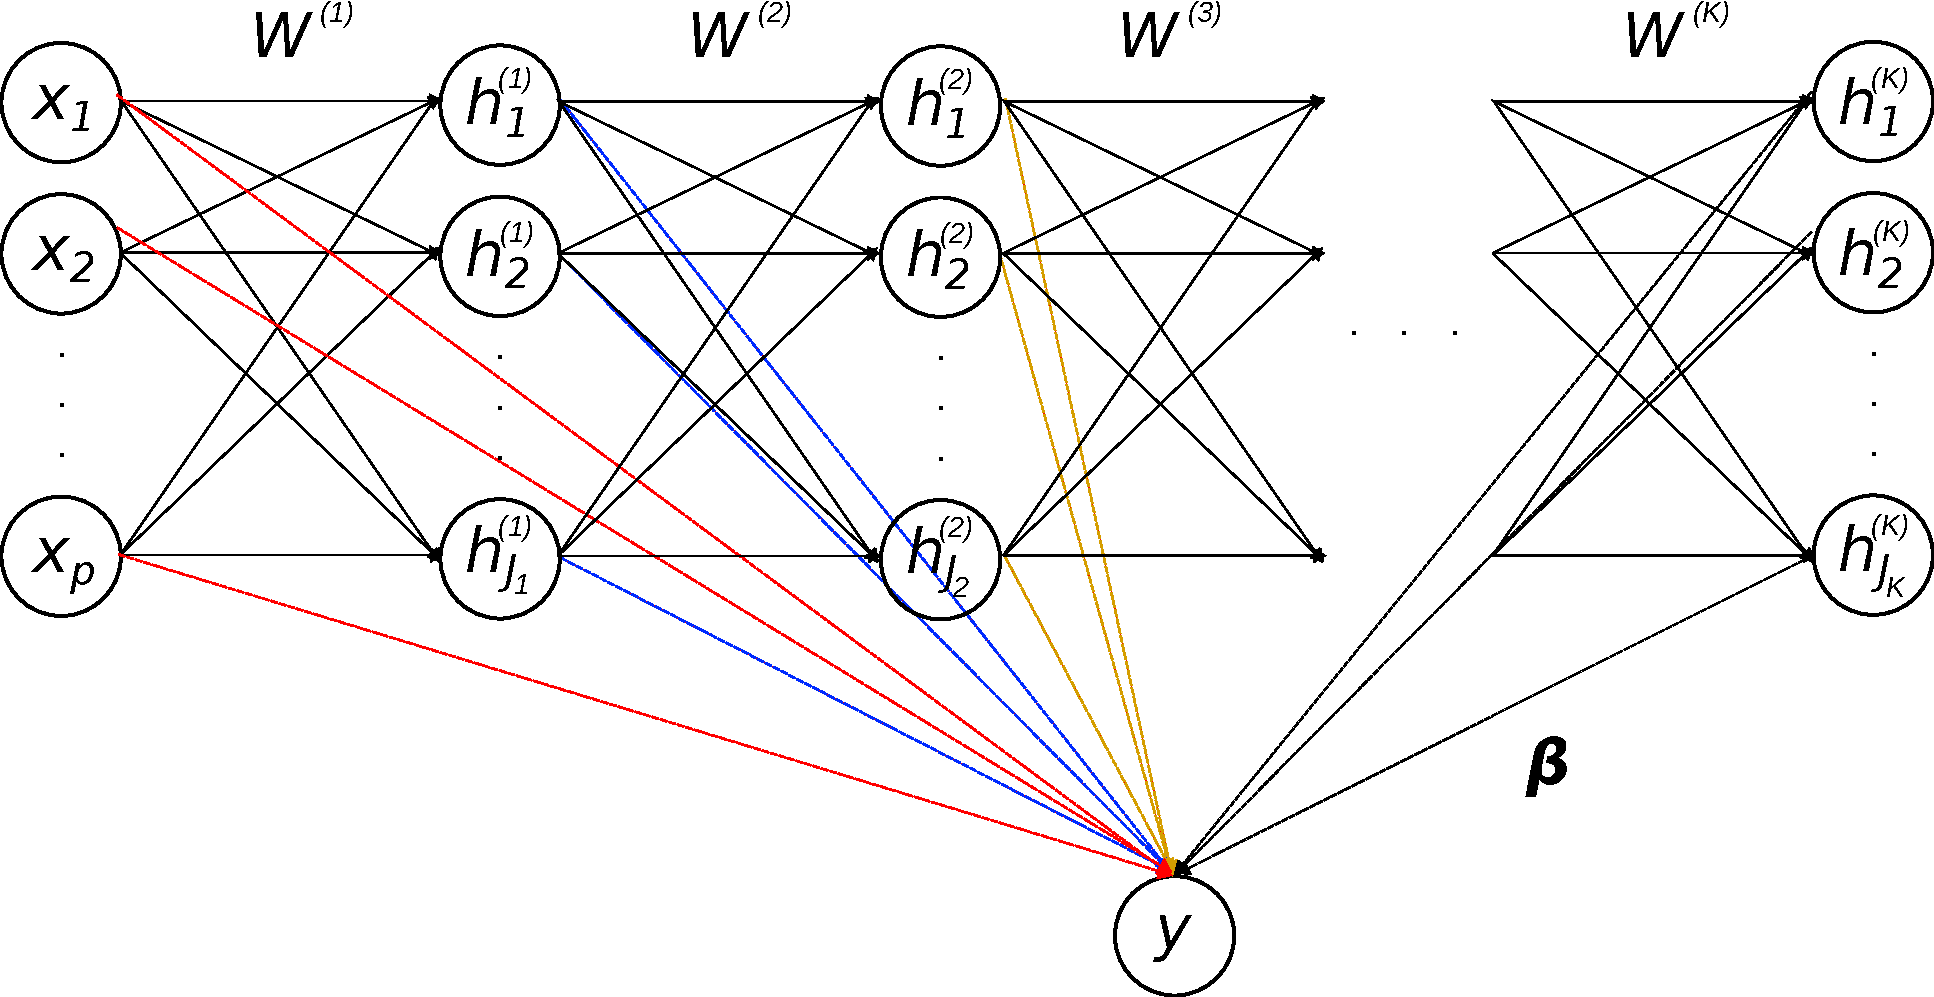
\includegraphics[width=0.45\linewidth]{./Figures/deepRWNNalt} 

}

\caption[Graph representation of a deep random weight neural network (RWNN) with functional link between the input-layer, intermediate hidden-layers, and the output-layer]{Graph representation of a deep random weight neural network (RWNN) with functional link between the input-layer, intermediate hidden-layers, and the output-layer.}\label{fig:deeprwnn}
\end{figure}
\end{CodeChunk}

The two structures depicted in Figure \ref{fig:deeprwnn}, yields four
options when constructing a deep RWNN:

\begin{itemize}
\item
  \(\boldsymbol{d}_n = \boldsymbol h_n^{(K)}\)
\item
  \(\boldsymbol{d}_n = [(\boldsymbol h_n^{(K)})^T \; \boldsymbol x_n^T]^T\)
\item
  \(\boldsymbol{d}_n = [(\boldsymbol h_n^{(1)})^T \; (\boldsymbol h_n^{(2)})^T \; \cdots \; (\boldsymbol h_n^{(K)})^T]^T\)
\item
  \(\boldsymbol{d}_n = [(\boldsymbol h_n^{(1)})^T \; (\boldsymbol h_n^{(2)})^T \; \cdots \; (\boldsymbol h_n^{(K)})^T \; \boldsymbol x_n^T]^T\)
\end{itemize}

Given a matrix \(D\), with its \(n\)'th row corresponding to
\(\boldsymbol{d}_n\), it follows that estimating the output-weights of a
deep RWNN is equivalent to that of the RWNN using only a single
hidden-layer.

Like the estimation process, sampling the hidden weights is similar to
that of RWNN's with a single hidden-layer. However, while the random and
random orthogonal initialisation methods can be performed independently
on a layer-by-layer basis, the quasi-random initialisation has to
continue its quasi-random sequence layer-to-layer (i.e.~the sequence is
not reset between layers).

The \pkg{RWNN} package allows the user to specify the number of neurons
and the activation function (found in Table \ref{tab:activation}) in
each of the \(K\) hidden-layers, as well as which of the four modelling
approaches should be taken (when nothing is specified it defaults to the
third option).

\hypertarget{sparse-rwnn}{%
\subsection{Sparse RWNN}\label{sparse-rwnn}}

\hypertarget{pre-trained-using-an-auto-encoder}{%
\subsubsection{Pre-trained using an
auto-encoder}\label{pre-trained-using-an-auto-encoder}}

\hypertarget{pruning-using-magnitude}{%
\subsubsection{Pruning using magnitude}\label{pruning-using-magnitude}}

\hypertarget{pruning-using-fisher-information}{%
\subsubsection{Pruning using Fisher
information}\label{pruning-using-fisher-information}}

\hypertarget{pruning-using-mutual-information}{%
\subsubsection{Pruning using mutual
information}\label{pruning-using-mutual-information}}

\hypertarget{ensemble-methods}{%
\subsection{Ensemble methods}\label{ensemble-methods}}

\hypertarget{stacking}{%
\subsubsection{Stacking}\label{stacking}}

\hypertarget{bagging}{%
\subsubsection{Bagging}\label{bagging}}

\hypertarget{boosting}{%
\subsubsection{Boosting}\label{boosting}}

\hypertarget{ensemble-deep-rwnn}{%
\subsubsection{Ensemble Deep RWNN}\label{ensemble-deep-rwnn}}

\hypertarget{EX}{%
\section{Examples}\label{EX}}

\hypertarget{CON}{%
\section{Conclusions}\label{CON}}

\renewcommand\refname{References}
\bibliography{literature.bib}



\end{document}
